In Section \ref{subsec:fgrPCA} \ac{PCA} was used used to show that three eigenvectors are sufficient to capture over 99\% of the variance in Bison's simulated Ris\o~ AN3 power ramp fission gas release time series. The variation is caused by perturbations in the fission gas release parameters although they are not explicit in the \ac{PCA} framework. The Dakota code is used to create the 100 time series in the previous section. In accordance with each parameter's uniform distribution described in Table \ref{table:fgr_params}, Dakota made 100 sets of perturbations to the parameters using the \ac{LHS} method. Each of the 100 samples was then propagated through Bison and a time series of fission gas release was output. \ac{PCA} was then performed on the covariance matrix of the 100 samples. Consequently, there is a clear mapping from a set of eight fission gas release parameters to a time series. More specifically, there is a mapping from the i$^{th}$ set of eight parameters $R^{i}$ to the three expansion coefficients $\lbrace p_{i1}, p_{i2}, p_{i3} \rbrace$ that are capable of reproducing the time series, as described in Eq. \ref{eq:pcaExpCoeffs}. In order to predict new time series for a set of fission gas release parameters not in the set used to derive the three principal components this mapping must be generated. Kriging is used achieve the mapping.  

To start, using the Kriging description in Section \ref{sec:kriging} a surrogate is constructed for each of the expansion coefficients related to the three principal components responsible for over 99\% of the variance. Each of these surrogates $\hat{p}_{ij}$ for $j\in\left(1,2,3\right)$ accepts a set of fission gas release parameters and outputs a scalar expansion coefficient for the principal component $X_j$. In accordance with Eq. \ref{eq:pcaExpCoeffs} the predicted fission gas release time series is,
\begin{equation}
\label{eq:predicted_mean_fgr_ts}
 \hat{\mathcal{F}}^{i}(R^i) = \hat{p}_{i1}\left(R^i\right) X_1 + \hat{p}_{i2}\left(R^i\right) X_2 + \hat{p}_{i3}\left(R^i\right) X_3 + \mu  
\end{equation}
where $\mu$ is the mean release time series of the 100 simulations. Since Kriging surrogates return an uncertainty $\sigma_{\hat{p}_{ij}}$ along with a predicted scalar value, an uncertainty band can be derived for the time series in Eq. \ref{eq:predicted_mean_fgr_ts}.
\begin{equation}
\label{eq:predicted_std_fgr_ts}
 \sigma_{ \hat{\mathcal{F}}^i }^2 = \sigma_{\hat{p}_{i1}}^2 X_1^2 + \sigma_{\hat{p}_{i2}}^2 X_2^2 + \sigma_{\hat{p}_{i3}}^2 X_3^2 
\end{equation}
The shape of the uncertainty vector output by Eq. \ref{eq:predicted_std_fgr_ts} is equal to the number of time-steps utilized in the principal components. 

\subsubsection{Cross Validation}
\label{subsec:cross_validation}

With a Kriging formulation for predicting Ris\o~ AN3 power ramp fission gas release time series for any set of Bison fission gas release parameters in place, it is necessary to test the formulation. In other words, it's necessary to investigate the error in the formulation's predictions. If the Kriging surrogates can accurately predict their respective \ac{PCA} expansion coefficients then the formulation will be able to accurately predict gas release time series since Eq. \ref{eq:predicted_mean_fgr_ts} is just a linear combination of the predictions. To this end, a test set of 100 independent Bison simulations of the Ris\o~ AN3 power ramp were obtained. The simulations in the test set are completely isolated from those in the training set and not used in calculating the Kriging surrogates nor the principal components. There are several common approaches to judging the validity of a predictive model as described in \cite{Jones_Schonlau}. With training and test sets available at disposal are true expansion coefficient values, predicted values, and uncertainties in the predicted values. Using these components the standardized cross-validated residual is defined as,
\begin{equation}
\label{eq:stnd_xval_residual}
 \frac{ p_{ij} - \hat{p}_{ij} }{ \sigma_{\hat{p}_{ij}} } . 
\end{equation}  
The standardized cross-validated residuals for all three Kriging surrogates' predictions on the test set are shown in Fig. \ref{fig:xval_3sig_bands}. Note the Kriging models used to predict the expansion coefficients are built on 100 samples analyzed previously in Sec. \ref{subsec:fgrPCA}.  
\begin{figure}
\caption{\label{fig:xval_3sig_bands}
Cross validation of Kriging predictions for \ac{PCA} expansion coefficients using 3$\sigma$ band approach.}
 \begin{center}
  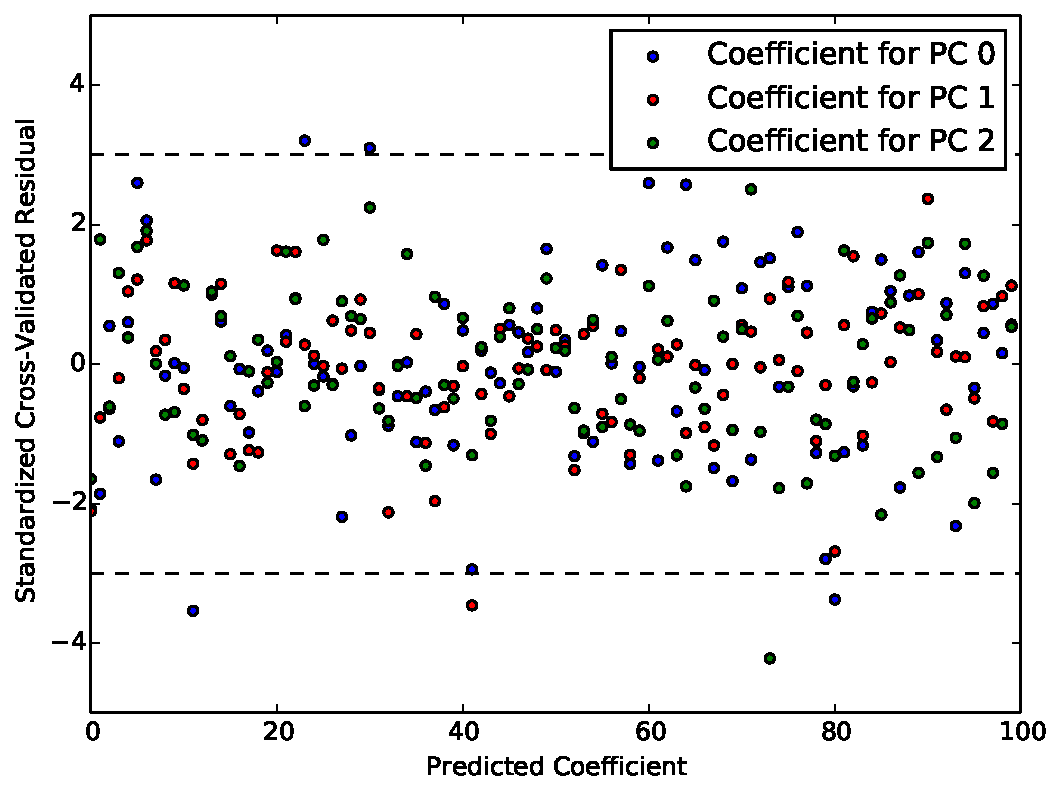
\includegraphics[scale=.75]{./Chapter4/xval_3sig_band.pdf}
 \end{center}
\end{figure}
Each point represents the number of standard deviations the true expansion coefficient is to the predicted coefficient. Some 99.7\% of points are expected to lie within the band $\left[-3, +3\right]$. Indeed, of the 300 points appearing in Fig. \ref{fig:xval_3sig_bands} some six lie outside the bands, which is a first indication that the predictive model has merit.  

In the second cross validation approach, the predicted values are plotted directly against the true values as shown in Fig. \ref{fig:xval_45degree}. Ideally, all points would lie on the 45$^{\circ}$ line, which would indicate that predictions perfectly match the true expansion coefficient values. The plots in Fig. \ref{fig:xval_45degree} show that the predicted values do generally approach this trend despite the presence of some noise. For predictions of each expansion coefficient in Fig. \ref{fig:xval_45degree} the results are plotted when 20, 60, and 100 random samples from the test set are utilized. Of course, less noise is present as the number of samples used to build the surrogates increase.  
\begin{figure}
\caption{\label{fig:xval_45degree}
Cross validation of Kriging predictions for \ac{PCA} expansion coefficients using 45$^\circ$ approach.}
 \begin{center}
  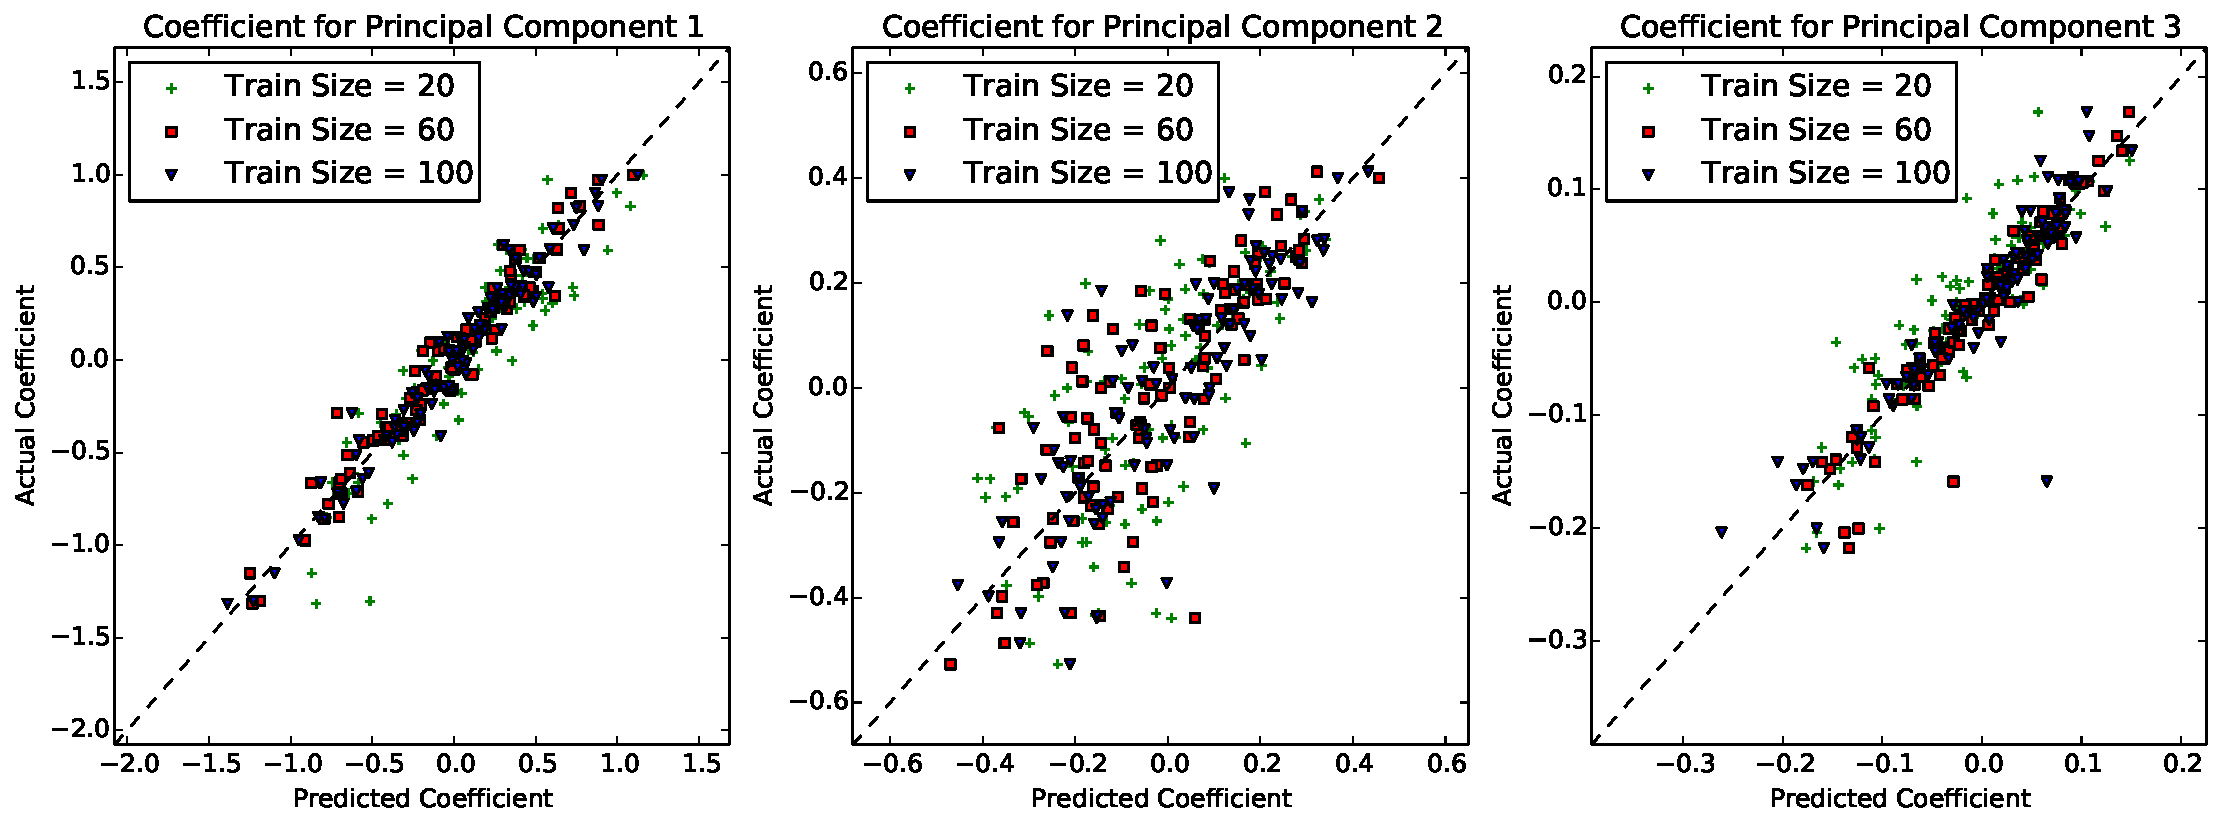
\includegraphics[scale=.4]{./Chapter4/xval_45degree.pdf}
 \end{center}
\end{figure}
Surprisingly, regardless of the training set size, predictions for the first principal component expansion coefficient are of the highest quality followed by the predictions for the expansion coefficients of the third principal component. It is most important to accurately predict expansion coefficients for the top principal components since they explain the most variance. Accurate prediction of lower principal components offers diminishing returns. Both inverse and logarithmic transforms were applied to the data as suggested in \cite{Jones_Schonlau} although no noticeable improvement was observed in prediction accuracy. Due to the relatively noisy values for the second expansion coefficient in Fig. \ref{fig:xval_45degree} it is anticipated the largest prediction errors will occur from the release jump and onwards since the second principal components attempts to account for a majority of the variance in this area per Fig. \ref{fig:fgrEvecs}.

\subsection{Calibration}
\label{subsec:calibration}

Now that the predictive accuracy of the individual Kriging surrogates for each expansion coefficient have been cross validated it is time to investigate how well the surrogates can perform collectively in predicting Ris\o~AN3 power ramp fission gas release time series. To determine the error between predicted time series the \ac{RMSE} is used as a cost function. Recall that before any two time series are compared each is segmented into 150 identical locations. The objective of calibration is to find a set of fission gas release parameters $R^i$ such that when they are input into Eq. \ref{eq:predicted_mean_fgr_ts} the \ac{RMSE} is minimized. 

Ideally, the landscape of possible \ac{RMSE} values is such that a clear global minimum exists. In this case, an algorithm such as \ac{EGO} can be used to find the minimal value and its corresponding parameter set \cite{Jones_Schonlau}. \ac{EGO} couples a computer model's surrogate prediction and uncertainty with the computer model itself in an iterative optimization process.  At each iteration \ac{EGO} estimates the parameter space location that is most likely to contain a \ac{RMSE} value smaller than the current minimum. The true computer model is then evaluated at this point and therefore, the minimization procedure can be potentially expensive. However, if it is known a priori that the \ac{RMSE} landscape is for example, convex then \ac{EGO} should be strongly considered. Unfortunately, there is usually no way to tell a priori the shape of a landscape for most expensive engineering codes such as Bison. Due to the non-linearities inherent in such codes the landscape is often fairly "flat". A flat landscape can result when some parameters are insignificant and thus, many values of these parameters will result in similar cost function values. Also, a flat landscape can result if the minimization problem is non-unique, meaning many combinations of parameters can yield the same, or nearly the same, optimal values for the \ac{RMSE}. Often times, these two issues may be interrelated and both will tremendously complicate the global optimizer search. Indeed, if \ac{EGO} is used many expensive computer code evaluations will be wasted. A local optimization algorithm should be utilized if a flat landscape is suspected.  

To decide which class of minimization algorithm to apply to solve the problem in-hand Sobol indices are calculated using the surrogate model. However, Morris' algorithm is first applied to get a sense of which of the eight fission gas release parameters in Table \ref{table:fgr_params} most influence the \ac{RMSE}. In reference to Section \ref{subsec:morris_algorithm}, 500 elementary effects are calculated for each fission gas release parameter. A total of 4500 evaluations of the surrogate in Eq. \ref{eq:predicted_mean_fgr_ts} were required to produce the plot in Fig. \ref{fig:fgr_morris_plot}.    
\begin{figure}[!h]
\caption{\label{fig:fgr_morris_plot}
Morris' algorithm applied to the \ac{RMSE} of the fission gas release time series.}
 \begin{center}
  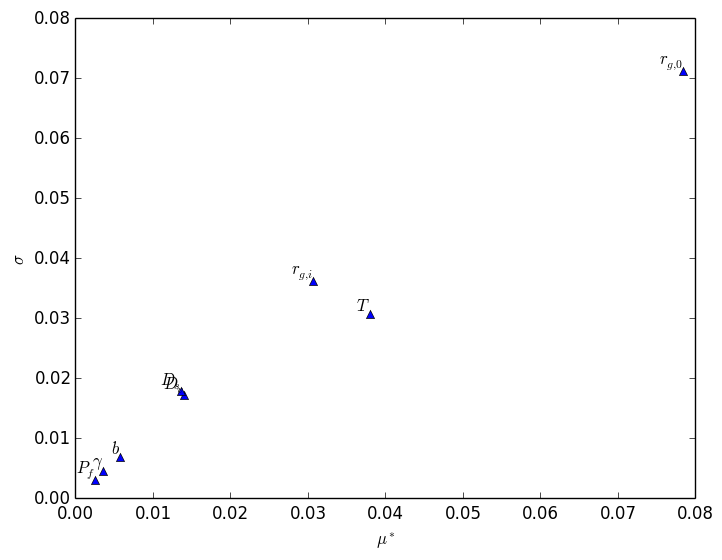
\includegraphics[scale=.75]{./Chapter4/fgr_morris.png}
 \end{center}
\end{figure}
The value $\mu^*$ in Fig. \ref{fig:fgr_morris_plot} is simply the average of the absolute values of each parameter's elementary effects, as defined in Eq. \ref{eq:elementary_effect_x}. Taking the absolute value helps to ensure cancellation effects in non-monotonic models do not obscure a parameter's true influence \cite{Morris}. The initial fuel grain radius is clearly the most influential parameter followed by the fuel grain and temperature scaling parameters. Such results are consistent with the variable importances discovered through the \ac{PCA} study that resulted in Fig. \ref{fig:principalCompTS}. The importance of fuel grain radius parameters is of no surprise given how omnipresent they are in the \ac{SIFGRS} model, and specifically in determining diffusion distances and grain boundary sweeping. The positive distances away from the origin along the $\sigma$-axis are indicative of non-linear interaction effects between the fission gas release parameters and a first sign that a global minimum solution may be too computationally expensive for the calibration problem.  

Further investigation of the sensitivity of the \ac{RMSE} with respect to its input parameters is achieved by calculating Sobol indices. As described in \cite{Sobol}, Sobol indices attribute a system's total variance to individual variables and their interactions with other variables by applying the anchored-\ac{ANOVA} decomposition described in Section \ref{subsec:anchored_anova}. In reference to Eq. \ref{eq:hdmr_decomp}, the "main effect index" is defined to be the variance of $f_\textbf{u}\left(\textbf{x}_\textbf{u}\right)$ normalized by the system's total variance. The main effect determines the fraction of variance that is due to either one variable or any number of interacting variables. The anchored-\ac{ANOVA} frameworks allows for the subtraction of variance contributions from other variables. If the main effect indices are added for all combinations of a systems $d$ variables then the $2^d-1$ components are expected to sum to unity. 

However, the integrals involved in calculating the variance of $f_\textbf{u}\left(\textbf{x}_\textbf{u}\right)$ are expensive and therefore, typically main effect indices are only calculated for the individual variables and not their interactions \cite{Saltelli}. The "total effect index" uses the anchored-\ac{ANOVA} decomposition to estimate the variance due to a variable and all of its possible interactions with other variables in the system. The calculation of total effect indices is made possible thanks to the total variance theorem \cite{Saltelli}. Unlike the sum of all main effect indices, the sum of all total effect indices is expected to sum to unity only when the model under consideration is purely additive.  

Various methods exist for computing Sobol indices, all of which are based on the Monte Carlo method for estimating the integrals in the variance calculations when the model under consideration is not analytic. The R code package \cite{R} is utilized for calculating Sobol indices for the problem in hand. Specifically, the method of Sobol and Jansen \cite{Saltelli} is used initially to estimate main and total effect indices. The Sobol and Jansen algorithm requires $n(d+2)$ evaluations of the objective function to estimate both sets of indices, where $n$ is the number of Monte Carlo samples to use. Both main and total effect indices for the \ac{RMSE} are displayed in Fig. \ref{fig:rmse_sobol_indices} using $10^5$ Monte Carlo samples and 100 bootstrap samples to obtain $95\%$ confidence intervals. 
\begin{figure}[!h]
\caption{\label{fig:rmse_sobol_indices}
Main and total effect indices for the \ac{RMSE} using the Sobol-Jansen algorithm. A total of $n=10^4$ Monte Carlo samples are used to estimate the indices.}
 \begin{center}
  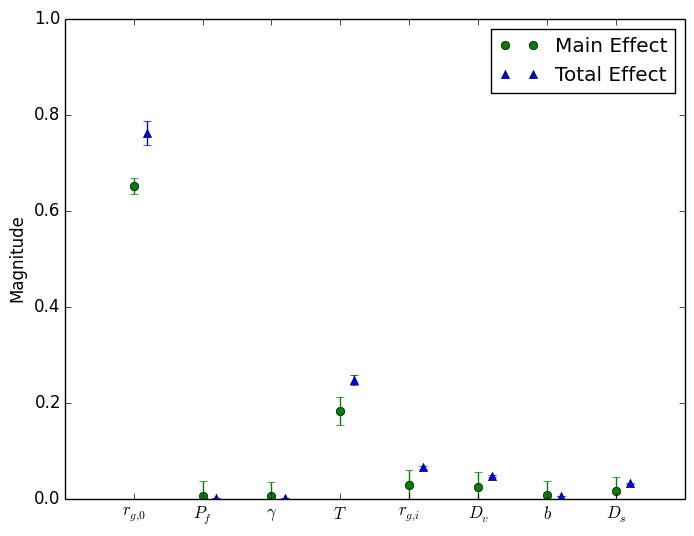
\includegraphics[scale=.75]{./Chapter4/sobol_indices.png}
 \end{center}
\end{figure}
Note, a total of $10^5$ calculations for the \ac{RMSE} were required to produce the data in Fig. \ref{fig:rmse_sobol_indices}. Without a surrogate model, the Bison code would have to be executed this same number of times, which would be prohibitive. The main effect magnitudes for each of the eight fission gas release parameters is entirely consistent with Fig. \ref{fig:fgr_morris_plot}. The far greatest variance is due to the initial fuel grain radius followed by the temperature and fuel grain radius scaling factors. The intra-granular and vacancy diffusion coefficients have non-zero but relatively small Sobol sensitivity indices. However, $P_f$, $\gamma$, and $b$ contribute trivially to any variability in the \ac{RMSE}. From Fig. \ref{fig:rmse_sobol_indices} it is evident that the parameters with non-trivial main effect indices also have significant total effect indices. Consequently, higher-order parameter interactions play a significant role in determining the \ac{RMSE}. Such a discovery is no surprise given how, for example, tightly coupled the temperature and fuel grain radius are in the \ac{SIFGRS} formulation described in Section \ref{sec:fgrTheory}.

In order to get a sense for which fission gas release parameters are strongly interacting, second-order Sobol indices are calculated in R. As seen in Fig. \ref{fig:rmse_sobol_indices_2nd_order} the highest magnitude interaction effects are between parameters with the largest main effects from Fig. \ref{fig:rmse_sobol_indices}. The largest interaction variance is due to the initial fuel grain radius and temperature scaling factor. Relatively large interactions that contribute to \ac{RMSE} variance are between the initial fuel grain radius and all the other fission gas release parameters. Of particular note is the magnitude of interaction between the vacancy diffusion coefficient and the temperature and initial fuel grain radius.     
\begin{figure}[!h]
\caption{\label{fig:rmse_sobol_indices_2nd_order}
Second order Sobol indices for the \ac{RMSE}. A total of $n=10^4$ Monte Carlo samples are used to estimate the indices.}
 \begin{center}
  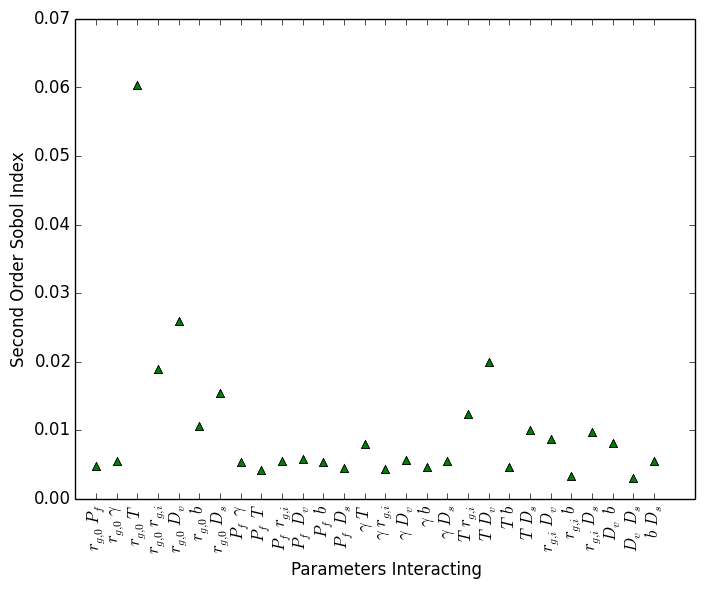
\includegraphics[scale=.75]{./Chapter4/sobol_2nd_order.png}
 \end{center}
\end{figure}
A total of $3.7\times 10^5$ \ac{RMSE} calculations were required to produce Fig. \ref{fig:rmse_sobol_indices_2nd_order}. As mentioned previously, such an analysis is only feasible using an efficient surrogate.

Given the presence of strong interaction among the fission gas release parameters it is unlikely a global \ac{RMSE} minimum can be found in reasonable time. However, a locally optimal solution can be found using the \ac{COBYLA} algorithm. The \ac{COBYLA} algorithm is of the simplex variety that does not require any gradient information while allowing for constraints to be placed on both the search parameters and objective function. For this problem it is necessary to not allow fission gas parameters that result in negative fission gas release values in predicted time series. Simplex algorithms are based on the fact that parameter constraints act as hyperplanes in d-dimensional space that collectively enclose a convex volume. The optimal objective function value must lay on one of the vertices of the intersection of the hyperplanes \cite{Powell}. 

Since local optimization algorithms such as \ac{COBYLA} are notorious for being sensitive to initial search conditions the algorithm is executed 100 different times, with each execution being seeded by one of the 100 \ac{LHS} used to construct the expansion coefficient surrogates. Such a procedure increases the probability of finding a true minimum \ac{RMSE} and not one existing in a flat space. The minimum \ac{RMSE} found was 0.02941, which corresponded to the predicted time series in Fig. \ref{fig:fgr_best_estimate}. 
\begin{figure}[!h]
\caption{\label{fig:fgr_best_estimate}
Best-estimate fission gas release time series compared to experimental data.}
 \begin{center}
  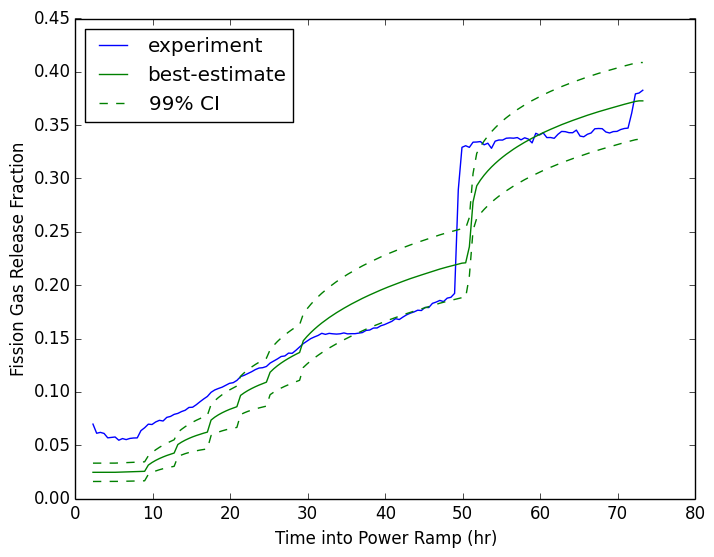
\includegraphics[scale=.75]{./Chapter4/fgr_best_estimate.png}
 \end{center}
\end{figure}
To identify the locally minimum \ac{RMSE} some $10^5$ instances of the surrogate were required. For each of the 100 seedings the \ac{COBYLA} algorithm was terminated either after $2\times 10^3$ iterations or a relative difference of $10^{-6}$ between two consecutive iterations. While the time series in Fig. \ref{fig:fgr_best_estimate} is certainly an improvement over the time series produced when the mean fission gas parameter values are used in Fig. \ref{fig:riso_fgr}, the predicted fission gas release time series leaves much to be desired. Discrepancies between predicted and experimental values may safely be attributed to the way in which gas release is modeled in \ac{SIFGRS}. The optimal parameter values, with each parameter scaled to the unit hypercube, found for each of the 100 \ac{COBYLA} seedings is summarized in a boxplot in Fig. \ref{fig:optimal_params_boxplot}.    
\begin{figure}[!h]
\caption{\label{fig:optimal_params_boxplot}
Boxplot of optimal parameter combinations for 100 seedings of the \ac{COBYLA} algorithm.}
 \begin{center}
  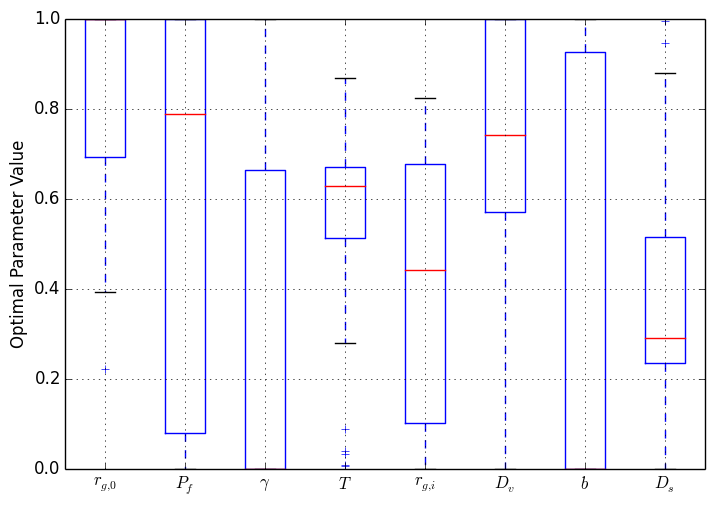
\includegraphics[scale=.75]{./Chapter4/optimal_params_boxplot.png}
 \end{center}
\end{figure}
The length of the whiskers in Fig. \ref{fig:optimal_params_boxplot} implies strong non-linear interaction effects, as substantiated by the investigation involving Sobol indices. The relative difference between the maximum \ac{RMSE} and minimum \ac{RMSE} among all 100 optimized seedings was only some 35\%. The relatively low differences between the two extremes was achieved using a wide combination of parameter values.  

One path taken to lessen the difference between experimental data and prediction was to smooth the experimental data. As mentioned previously, the measurements taken of fission gas release during the Ris\o~ AN3 power ramp may contain significant error. At some points in the experimental data the total fission gas release actually decreases, which is completely not physical. However, with only a single time series measurement there is no way of assigning uncertainties to fission gas release values measured at different times throughout the power ramp. Also, it would be unfounded to assign an uncertainty of say, 10\% to all measurements taken during the power ramp. Consequently, in an attempt to smooth the experimental data local polynomial regression was applied with the minimal amount of smoothing necessary to make the fission gas release time series strictly monotonically increasing. Using the R "loess" function with linear interpolants and a spanning parameter of 0.17 the desired smoothing was achieved. The smoothed experimental data along with the best-fit surrogate prediction is shown in Fig. \ref{fig:best_estimate_smooth}.  
\begin{figure}[!h]
\caption{\label{fig:best_estimate_smooth}
Best-estimate fission gas release time series compared to experimental data that was smoothed using the local polynomial regression smoothing.}
 \begin{center}
  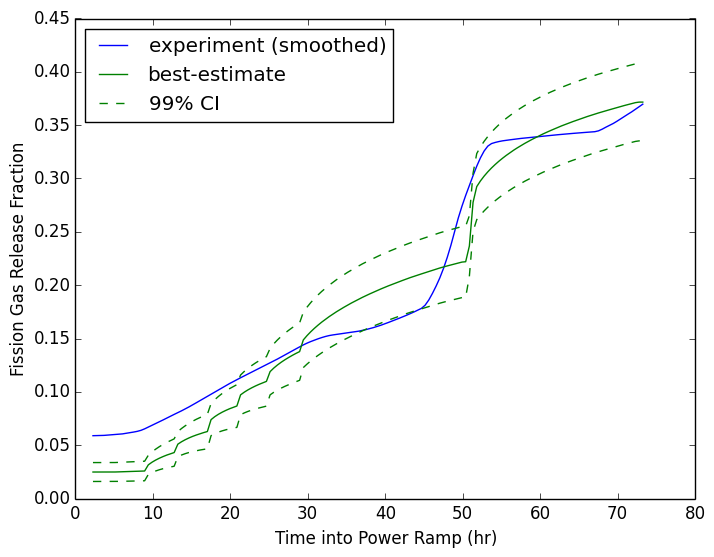
\includegraphics[scale=.75]{./Chapter4/best_estimate_smooth.png}
 \end{center}
\end{figure}
The \ac{RMSE} for the best-estimate time series when compared to the smoothed experimental data was calculated to be 0.02486, which was a 15.5\% reduction in \ac{RMSE} from when raw experimental data was utilized.

Comparing Fig. \ref{fig:best_estimate_smooth} with  Fig. \ref{fig:fgr_best_estimate}, it is not clear whether the smoothed experimental data offers any advantages towards finding a set of Bison fission gas release parameters that best predict the available data. Although there are significant discrepancies between predicted and experimental time series, especially in the power burst occurring at hour fifty of the power ramp, the Bison predictions do a good job in predicting end-of-experiment fission gas release values. For the case when raw experimental data is used, as in Fig. \ref{fig:fgr_best_estimate}, there is only a 2.6\% relative error in the end-of-experiment fission gas release prediction. The beginning-of-experiment prediction error in this case is 64.8\%. For the case of smoothed experimental date the prediction results are marginally improved with a beginning-of-experiment prediction error of 57.8\% and an end-of-experiment error of 0.5\%. Note, it's possible to enforce the conditions of matching the predicted beginning-of-experiment and end-of-experiment predictions to their respective experimental values in the \ac{COBYLA} framework. However, the \ac{COBYLA} algorithm is unable to converge to a solution that matches these conditions. Enforcing only one of the conditions to a tolerance of $10^{-3}$ was achievable although the resulting solution grossly over predicted the fission gas release elsewhere in the time series. A table of calibrated fission gas release parameters for both raw and experimental data is summarized in Table \ref{table:optimal_fgr_paramaters}.        
\begin{table}[!h] 
\caption{Calibrated fission gas release parameters with respect to raw and smoothed experimental data.}
\label{table:optimal_fgr_paramaters} 
\centering
\begin{tabular}{||c|c|c|c|c||} 
\hline \hline
\textbf{Description} & \textbf{Symbol} & \textbf{Smoothed} & \textbf{Raw} & \textbf{Relative Difference} \\ \hline
Initial Fuel Grain Radius & $r_{g,0}$  & 1.50E-05 & 1.50E-05 & 0.0E+00 \\ \hline
Fuel Porosity               & $P_f$      & 0.10      & 0.09      & 8.2E-02 \\ \hline
Surface Tension           & $\gamma$  & 0.50     & 0.50      & 1.4E-04 \\ \hline
Temperature               & $T$          & 1.02   & 1.02     & 1.8E-04 \\ \hline
Fuel Grain Radius         & $r_g$       & 1.26     & 1.26      & 5.1E-03 \\ \hline
Vacancy Diffusion Coef.  & $D_v$      & 7.49      & 7.50     & 3.8E-04 \\ \hline
Resolution Parameter    & $b$         & 0.10      & 0.19     & 4.8E-01 \\ \hline
Intra-granular Diffusion Coef. & $D_s$ & 1.02 & 1.05   & 2.7E-02 \\ 
\hline \hline
\end{tabular}
\end{table}







 



   



    






   

